%%%%%%%%%%%%%%%%%%%%
%
% $Beschreibung: Einleitung in das Projekt "Demonstrator für einen Schrittmotor" $
% $Autor: Grönke $
% $Datum: 09.06.2024 $
% $Pfad: DemonstratorSchrittmotor/DeveloperDoc/Contents/de/Projektbeschreibung.tex $
% $Version: 2 $
%
%
%%%%%%%%%%%%%%%%%%%


\chapter{Projektbeschreibung}

\section{Aufgabenstellung}

Die Aufgabe besteht darin, mithilfe eines Arduino Nano 33 BLE Sense Lite einen Demonstrator für einen Schrittmotor zu entwickeln. Mittels einer Konstruktion, die über einen Schrittmotor verfügt, welcher einen Riemen antreibt, soll ein Schlitten auf einer Linearführung verfahren werden. Es sollen unterschiedliche Bewegungscharaketeristiken demonstriert werden. Durch die Programmierung des Arduino, wird der Schrittmotor gesteuert und wird in die gewünschte Richtung und Position bewegt. Dies beinhaltet eine korrekte Programmierung, sowie die korrekte Ausgabe durch den Schrittmotor und eine Konstruktion, die mit allen Teilen funktionsfähig ist. Nachfolgend wird die Hardware beschrieben, sowie die Entwicklung der Software und die Konstruktion und Fertigung des Demonstrators.

\section{Herausforderungen}

Das Projekt lässt sich in 3 verschiedene Teilprojekte unterteilen, die zum Abschluss der Aufgabe führen. Zuerst ist da die Programmierung und die Arbeit mit der Arduino IDE. Außerdem die Konstruktion des Demonstrators und zuletzt die hierfür benötigte Auswahl der Hardware-Teile. Ebenfalls wichtig ist der Umgang mit den elektronischen Bauteilen, dass diese nicht durch den elektrischen Strom beschädigt werden und das der Demonstrator für den Transport geeignet ist. 

\section{Lösungsansatz}
Durch die Ausarbeitung der Herausforderungen, können Lösungsansätze entwickelt werden. Vorab wurde eine erste Konzeptskizze angefertigt, aus der Ideen entstanden. Im ersten Konzept sollte der Schrittmotor eine Plattform über einen Riementrieb axial verfahren, erkennbar in Abbildung \ref{ErsteKonzeptskizze}. Dabei sollte der Verfahrweg der Plattform über einen Abstandssensor mit einem vorher definierten Abstand zu einem Objekt, geregelt werden. Wird das Objekt näher oder weiter entfernt vom Abstandssensor bewegt, verfährt die Plattform mit einem definierten Abstand mit. Alle vorhandenen Bauteile sollten an einem Alu-Profil befestigt werden.

\begin{figure}[htb]
	\begin{center}
		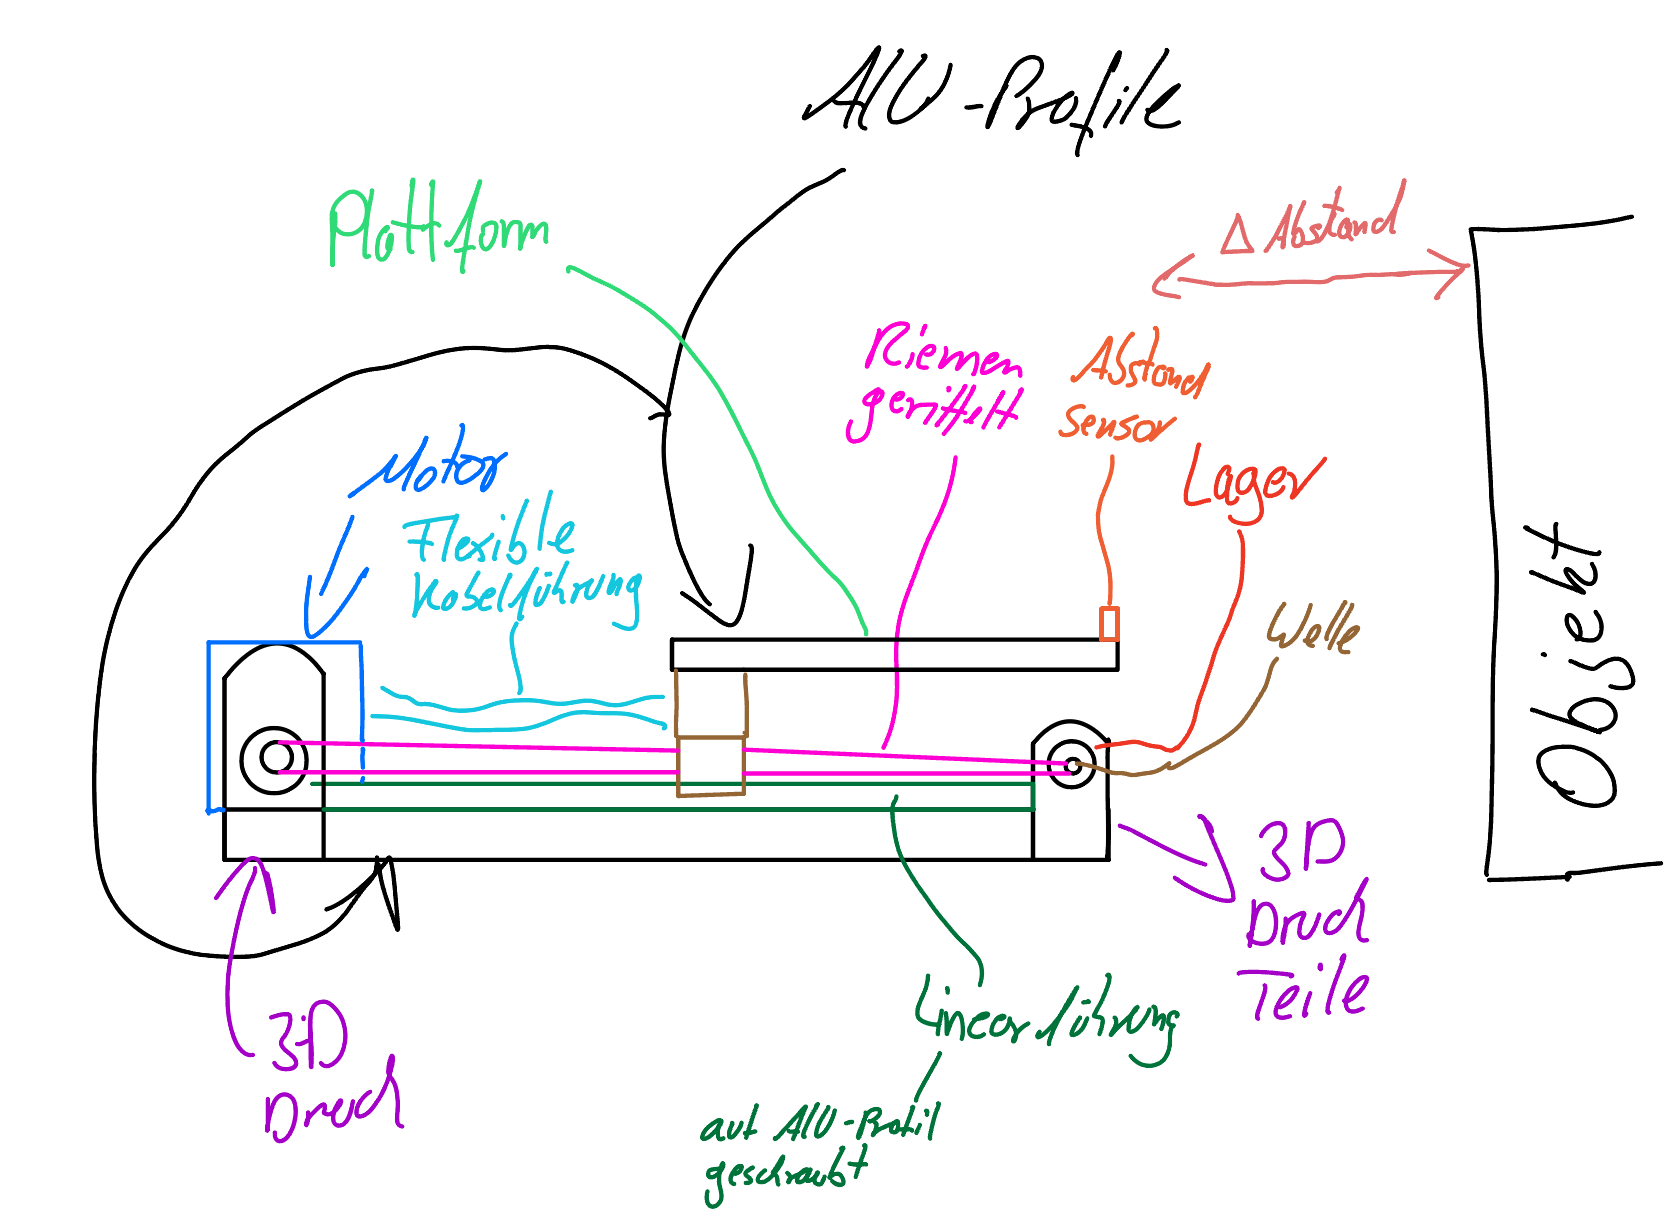
\includegraphics[width=\textwidth]{Images/Konzeptskizze1.png}
		\caption{Erste Konzeptskizze (Eigenaufnahme)} \label{ErsteKonzeptskizze}
\end{center}
\end{figure}

Aufgrund der hohen Komplexität wurde die Plattform inklusive des Abstandssensors, aus dem zweiten Konzept, erkennbar in Abbildung \ref{ZweiteKonzeptskizze}, entfernt. Stattdessen wird auf dem Schlitten der Linearführung ein Zeiger und auf dem Alu-Profil ein Lineal integriert. Mittels verschiedener Stufen soll der Schrittmotor unterschiedliche Bewegungsprofile demonstrieren. Vor allem sollte die Positioniergenauigkeit mit dem Zeiger dargestellt werden. Des Weiteren wurde ein Netzteil integriert, der sowohl den Motor als auch den Arduino mit Spannung versorgt. Außerdem ist ein Schalter zum Ein- und Ausschalten des Demonstrators, ein Stufenschalter zum Auswählen der Stufen sowie ein Taster zum Starten des Demonstrierablaufes eingebaut.  

\begin{figure}[H]
	\begin{center}
		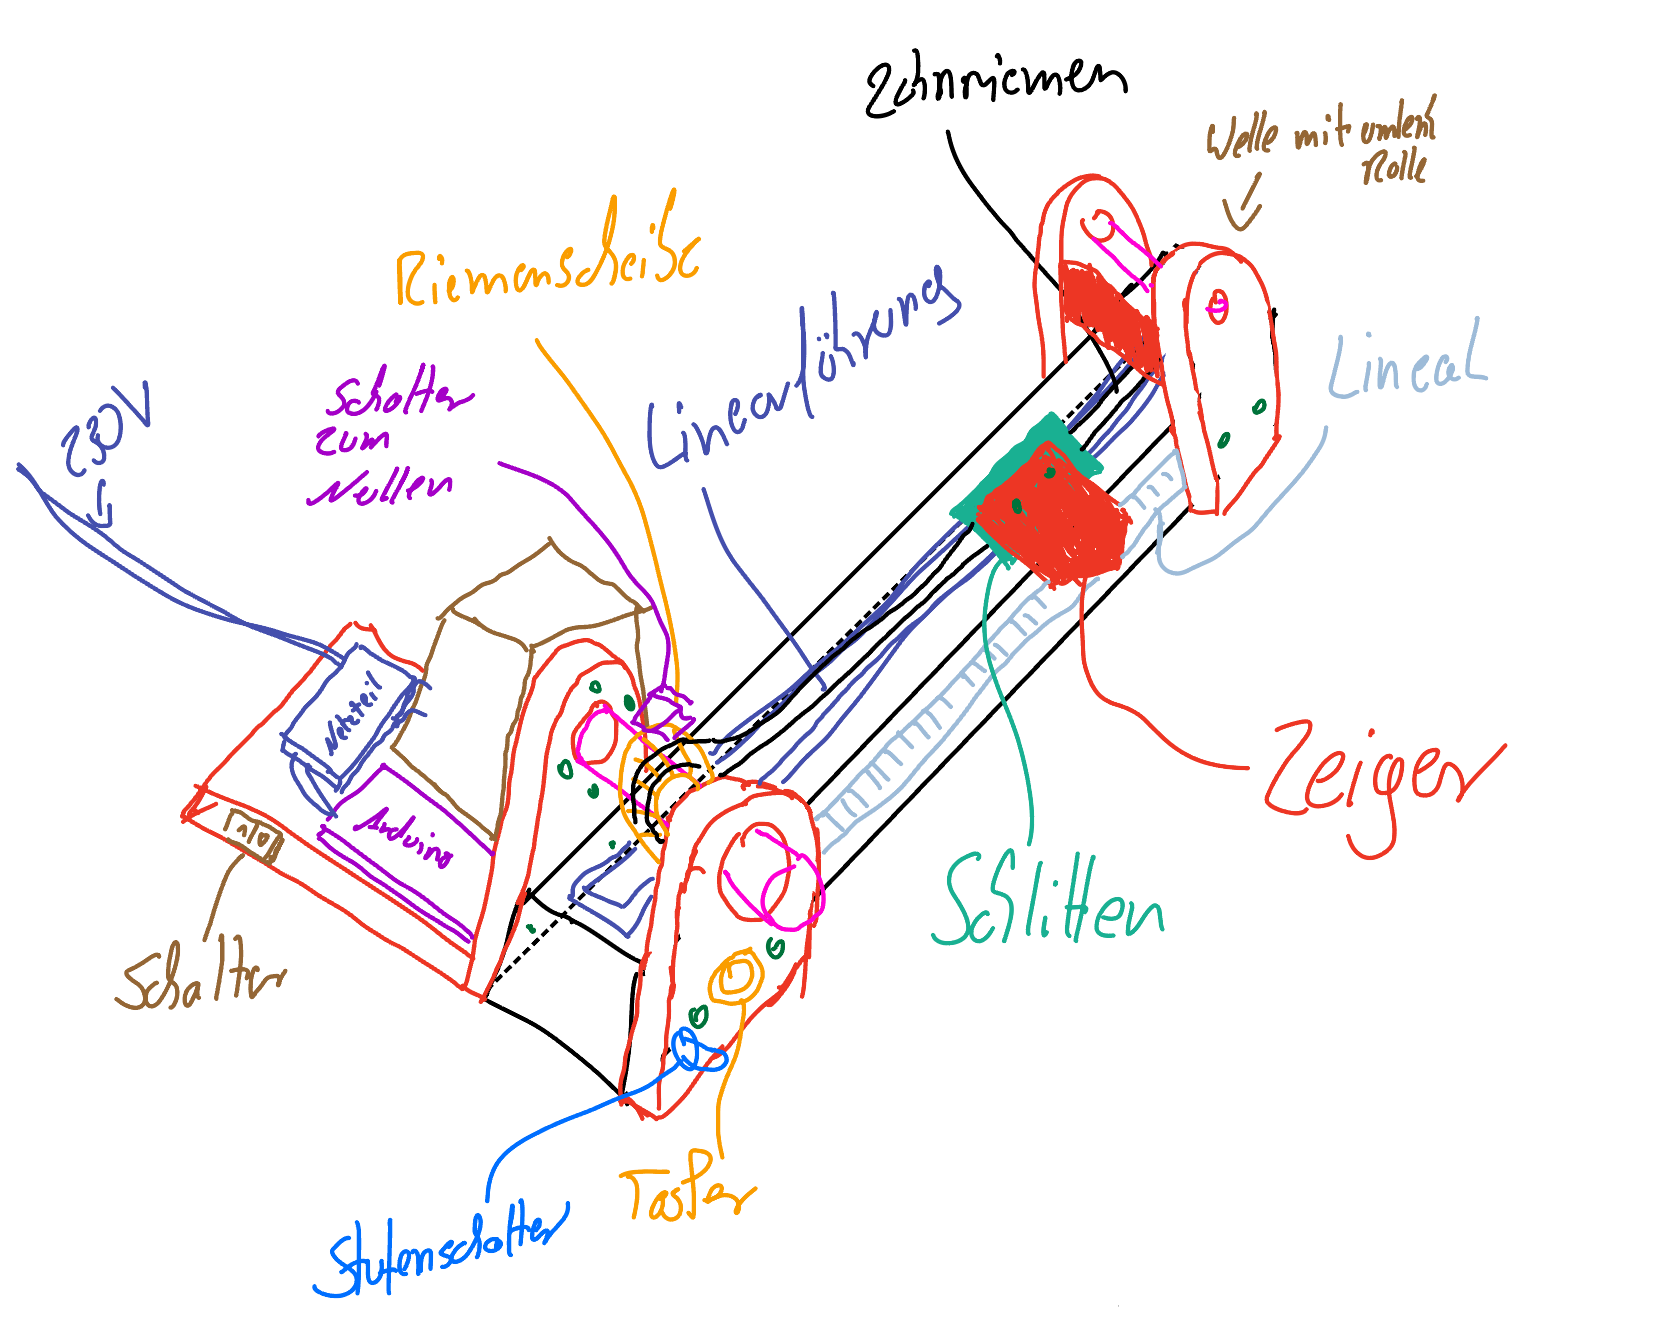
\includegraphics[width=\textwidth]{Images/Konzeptskizze2.png}
		\caption{Zweite Konzeptskizze (Eigenaufnahme)} \label{ZweiteKonzeptskizze}
	\end{center}
\end{figure}

Das zweite Konzept fand gefallen und wurde weiter durchdacht, sodass mit dem Handbuch angefangen werden konnte (siehe Handbuch Demonstrator für einen Schrittmotor). In diesem Handbuch sollte vor allem aus Kundenperspektive die einzelnen Funktionen und die Bedienung geklärt werden. Parallel konnte ein CAD-Modell konstruiert werden, erkennbar in Abbildung \Ref{CADMOD}. Gegenüber dem zweiten Konzept wurde die Hardware aus Transportiergründen mit auf dem Aluprofil verlegt und erhielt zum Schutz ein Gehäuse. Des Weiteren konnte eine Materialliste erstellt werden. 

\begin{figure}[H]
	\begin{center}
		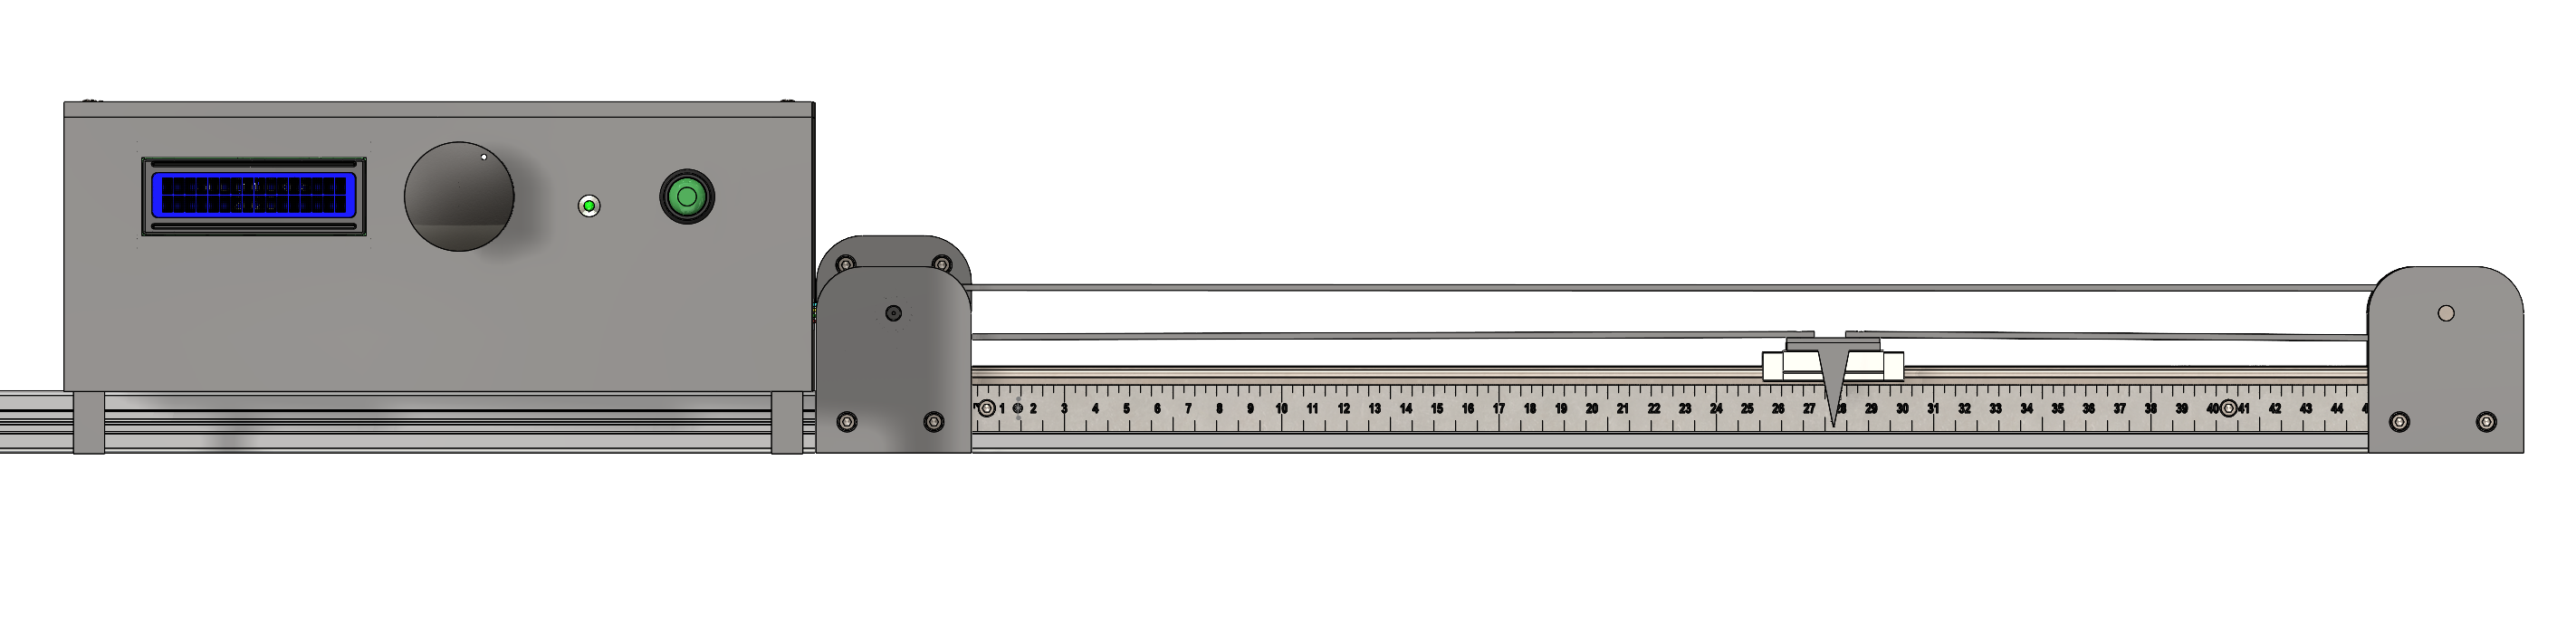
\includegraphics[width=\textwidth]{Images/Konstruktion1.png}
		\caption{CAD-Modell (Eigenaufnahme)} \label{CADMOD}
	\end{center}
\end{figure} 

%Durch die Ausarbeitung der Herausforderungen, können Lösungsansätze hierfür entwickelt werden. Indem vorab eine Skizze für die Konstruktion angefertigt wird, kann darauf basierend die Suche nach Teilen durchgeführt werden. Um den Demonstrator mit all seinen Teilen und seiner unhandlichen Größe trotzdem transportfähig zu konstruieren, werden die elektronischen Bauteile mit auf dem Alu-Profil montiert. Außerdem spielt es für die %Programmierung eine entscheidende Rolle, wie die verschiedenen Stufen angefahren werden sollen. Hierfür wurde sich von vornherein überlegt, wie die Stufen auszuwählen sind und in welche Positionen und in welchen Geschwindigkeiten verfahren wird.

\section{Anwendungsbereich des Projektes}

Der Demonstrator soll zur Veranschaulichung und als ergänzendes Lehrmittel dienen. So können Schüler oder Studierende die Prinzipien der Schrittmotorsteuerung, einschließlich der Schrittauflösung und Positionierung praxisnah erlernen. Des Weiteren können Studierende den Demonstrator dazu nutzen, um praktische Erfahrung zu sammeln zum Beispiel durch Programmierübungen. Außerdem könnte solch ein Demonstrator als Qualitätskontrolle dienen, um die Leistungsfähigkeit sowie die Genauigkeit von Schrittmotoren zu prüfen und sicherzustellen, dass sie den erforderlichen Spezifikationen entsprechen. Ein weiteres Anwendungsgebiet können Messen sein, da mit solch einem Demonstrator gut die Bewegungsabläufe und die präzise Positionierung gezeigt werden kann. 

\section{Besondere Herausforderungen bei den Quellen}

Eine der größten Herausforderungen in der Literaturrecherche lag darin, dass viele Datenblätter nicht in deutscher Sprache vorlagen. Diese mussten zunächst korrekt übersetzt werden, um sie dann interpretieren zu können. Ein hilfreiches Tool hierfür ist das Programm DeepL, womit ganze pdf-Dateien übersetzt werden können. Ein weiteres Problem bei der Ausarbeitung des Projektes war, dass trotz Nachfrage beim Hersteller kein Datenblatt für den verwendeten Schrittmotor erlangt werden konnte. Hierfür wurde ein Datenblatt eines vergleichbaren Schrittmotors herangezogen. Datenblätter sind für solch ein technisches Projekt essenziell, da sie technische Spezifikationen und wichtige Informationen zu der Funktionsweise und Einsatzmöglichkeiten liefern. Das dritte Problem, das sich uns während des Projektes geboten hat, ist das Fehlen von Daten wie beispielsweise einem Datum.


